\section[Pacote 2 - Servidor]{Pacote 2 - Servidor}
O pacote de estatísticas está relacionado à coleta de dados para a avaliação da quantidade de jogadores que usaram o jogos e dentre os que usaram, quais fases eles completaram e quantas vezes eles as completaram. O envio das estatísticas para o servidor não ocorrerá sem a ação do usuário, depende do jogador enviar os dados de acordo com a sua vontade de colaboração através de um botão na tela inicial e a confirmação do envio com a sua matrícula.

Ao se clicar no botão para enviar estatísticas do jogo, deve-se redirecionar para a tela igual a Figura \ref{envio_estatisticas}.


\begin{figure}[H]
\centering
\caption{Tela de envio de estatísticas}
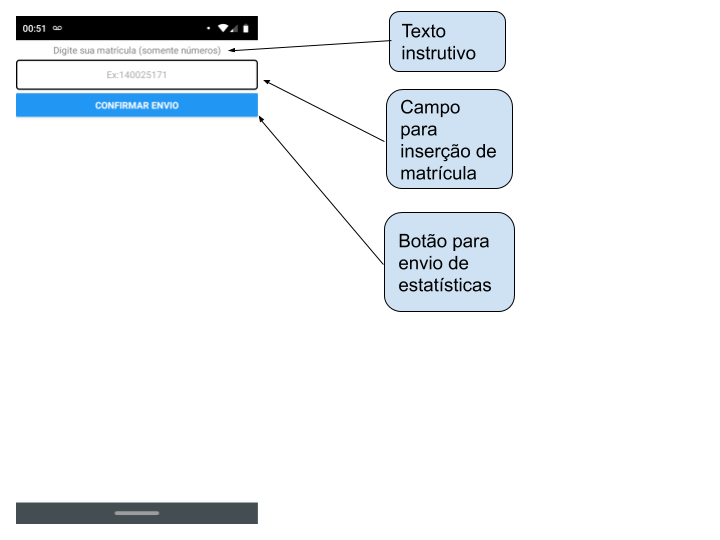
\includegraphics[scale=0.5]{figuras/estatisticas/envio_estatisticas.png}

\label{envio_estatisticas}
\end{figure}

A Figura \ref{matricula_incorreta} apresenta a mensagem de erro ao digitar a matrícula incorreta. A checagem é feita conferindo a quantidade de dígitos que deve ser igual a 8.


\begin{figure}[H]
\centering
\caption{Alerta de matrícula inválida}
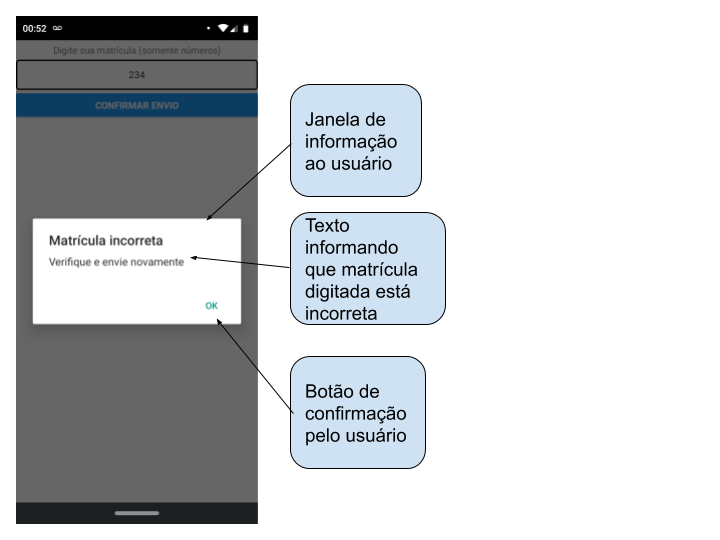
\includegraphics[scale=0.5]{figuras/estatisticas/matricula_incorreta.png}

\label{matricula_incorreta}
\end{figure}

A Figura \ref{sem_internet} apresenta a mensagem de erro quando não há conexão do celular com a internet para o envio dos dados ao servidor.

\begin{figure}[H]
\centering
\caption{Alerta de falta de internet}
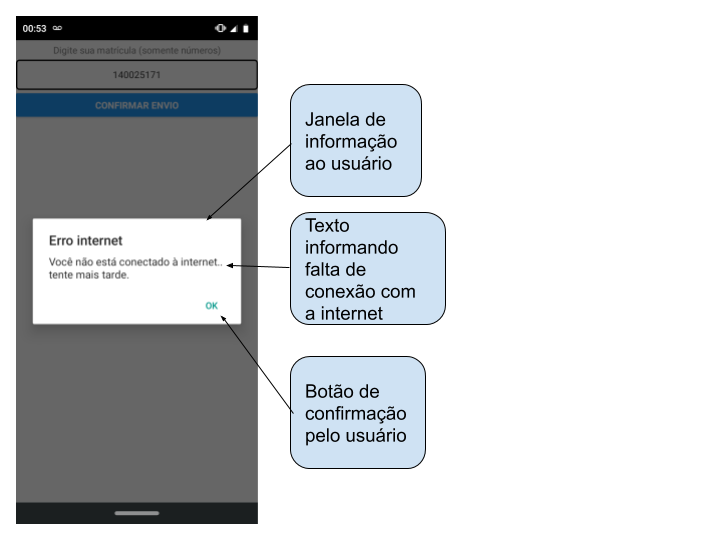
\includegraphics[scale=0.5]{figuras/estatisticas/sem_internet.png}

\label{sem_internet}
\end{figure}

Ao ser digitado a matrícula correta e realizada a submissão do envio das estatísticas, um loader aparecerá enquanto o procedimento não termina, como mostra a Figura \ref{loader} e ao terminar o envio, uma mensagem é apresentada, como mostra a Figura \ref{estatisticas_sucesso_envio}.

\begin{figure}[H]
\centering
\caption{Loader visível enquanto envia estatísticas}
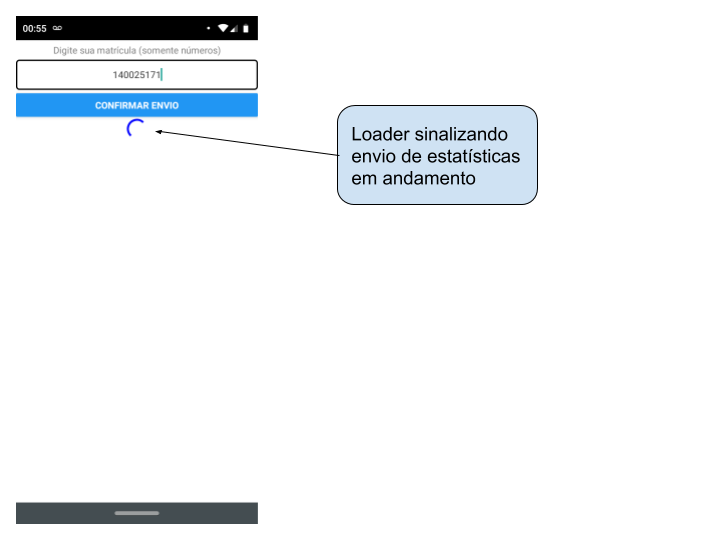
\includegraphics[scale=0.5]{figuras/estatisticas/loader_estatisticas.png}

\label{loader}
\end{figure}


\begin{figure}[H]
\centering
\caption{Alerta de envio com sucesso}
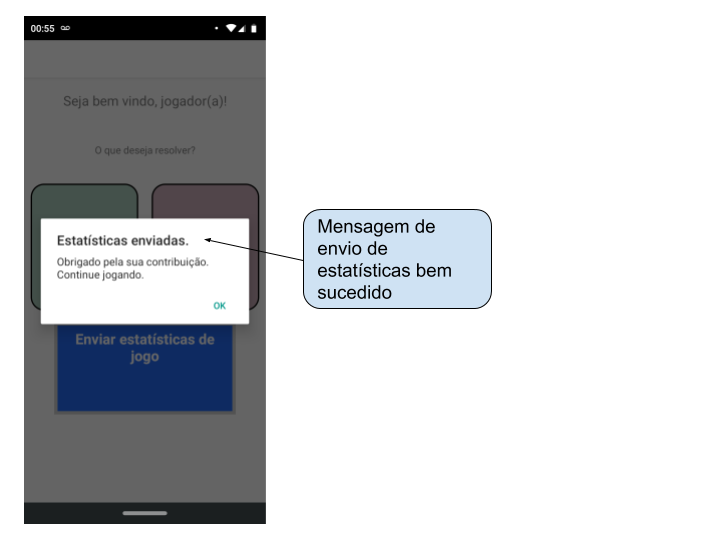
\includegraphics[scale=0.5]{figuras/estatisticas/estatisticas_enviadas.png}

\label{estatisticas_sucesso_envio}
\end{figure}

Ao fim do envio, é redirecionado para à tela inicial \ref{tela_inicial}.